\documentclass{article}
\usepackage[utf8]{vietnam}
\usepackage{graphicx}    % needed for including graphics e.g. EPS, PS
\usepackage{listings}
\usepackage{tikz}
\usetikzlibrary{calc}
\usepackage{tikz-cd}
\usetikzlibrary{positioning}
\usetikzlibrary{decorations.markings}
\usepackage{xifthen}
\usetikzlibrary{shapes.geometric}
\tikzset{main node/.style={rectangle,fill=white,draw,minimum size=1cm,inner sep=0pt},}
\tikzset{black node/.style={circle,fill=black,draw,minimum size=0.4cm,inner sep=0pt},}
\usepackage{color}
\usepackage{amsthm}
\usepackage{verbatim}
\usepackage{caption}
\usepackage{amssymb}
\usepackage{fullpage}
\usepackage{mathrsfs}
\usepackage{epstopdf}
\usepackage{framed,color}
\usepackage[top=1in, bottom=1in, left=1in, right=1in]{geometry}
\usepackage{float}
\linespread{1.3}
\restylefloat{table}
\usepackage[tikz]{bclogo}
\usepackage{wrapfig}
\usepackage[intlimits]{mathtools}
\usepackage{indentfirst}
\usepackage{mdframed}
\usepackage{commath}
\usepackage{soul}
\usepackage{enumerate}
\usepackage{mathabx}
\definecolor{dkgreen}{rgb}{0,0.6,0}
\definecolor{gray}{rgb}{0.5,0.5,0.5}
\definecolor{mauve}{rgb}{0.58,0,0.82}
\definecolor{shadecolor}{rgb}{1,0.8,0.3}
\topmargin -1.5cm
\oddsidemargin -0.04cm
\evensidemargin -0.04cm
\textwidth 16.59cm
\textheight 24cm
\parskip 7.2pt
\parindent 15pt
\DeclareMathOperator*{\esssup}{ess\,sup}
\newcommand*{\bigchi}{\mbox{\Large$\chi$}}% big chi
\newtheorem{vtheorem}{Định lý}
\newtheorem{vcorollary}{Hệ quả}
\newtheorem{vlemma}{Bổ đề}
\newtheorem{vproposition}{Tính chất}
\renewcommand*{\proofname}{Chứng minh}
\newtheorem*{vnote}{Ghi chú}

\title{Notes 3 tháng 7}
\author{Nguyễn Nga Nhi}

\begin{document}

\maketitle

\section{Long Short Term Memory}

Mục tiêu: learn from sequential data (language, visual, time series, planning)

* Vanila Recurrent Neural Networks

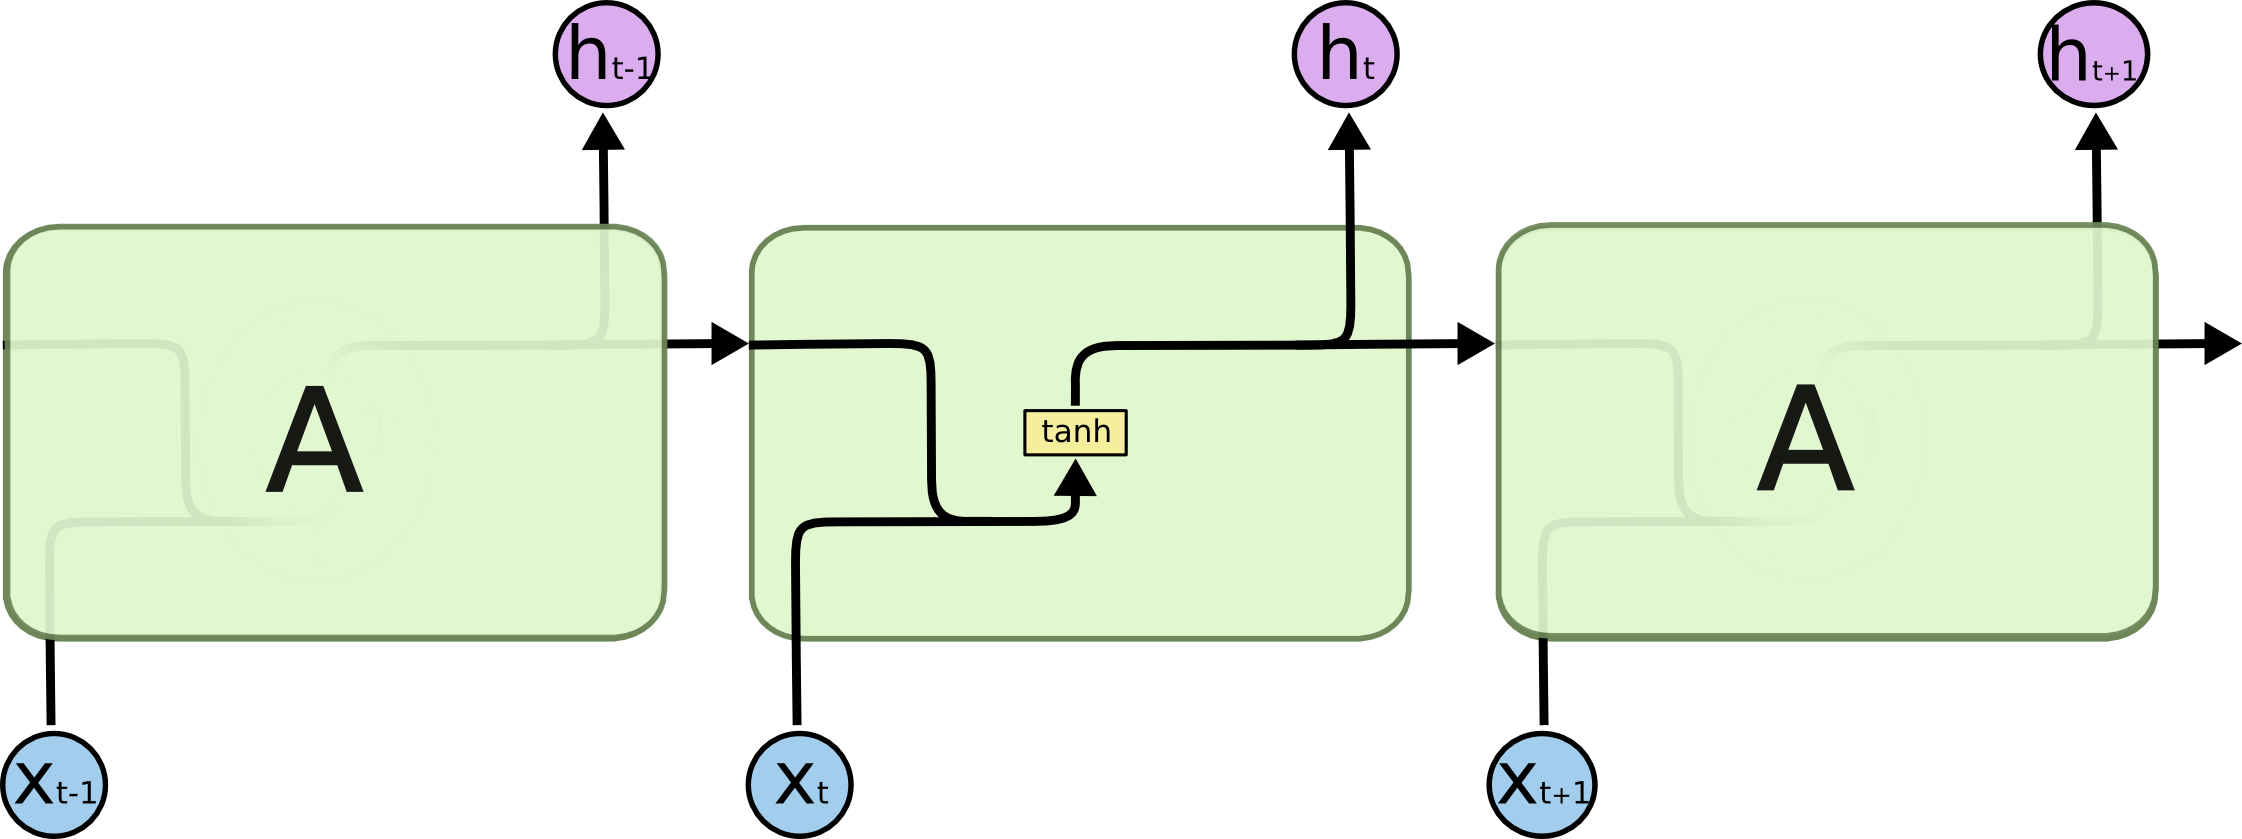
\includegraphics[width=300pt]{LSTM3-SimpleRNN.png}

+ (Stack RNNs

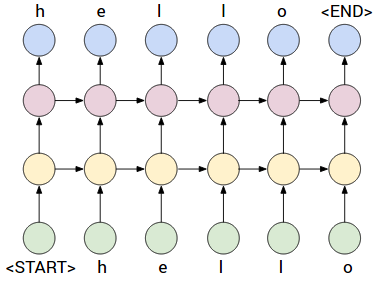
\includegraphics[width=300pt]{StackRNNs.png}

)

+ Issue with RNNs: No long-term memory

* LSTM

+ Important feature: Straight line cell state

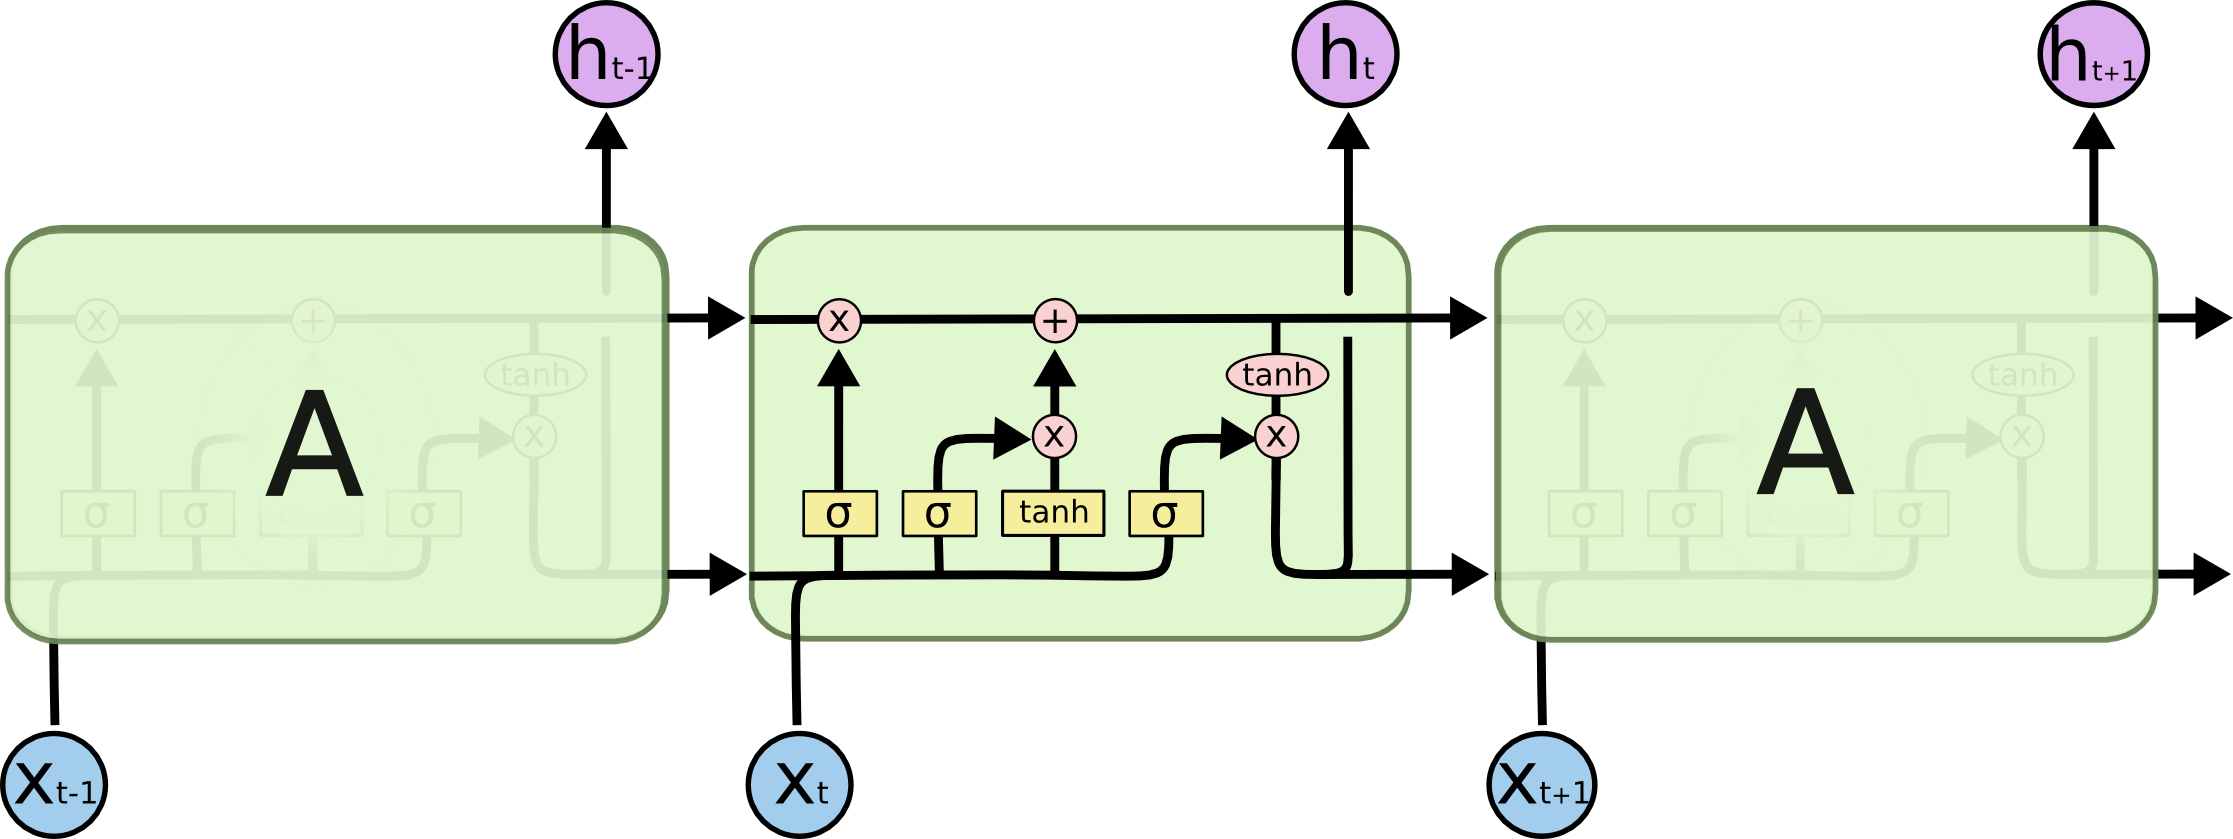
\includegraphics[width=500pt]{LSTM3-chain.png}

+ 3 additional gate layers: Forget, Input, Output

\textbf{forget gate layers}: nhớ hay không nhớ mỗi thông tin cũ

Sử dụng sigmoid $\implies$ độ cần thiết phải nhớ của mỗi thông tin cũ $\in$ [0,1]

\textbf{input gate layers}: lựa chọn ghi nhớ input nào

Xác định value vần update + Dựng vecto giá trị update $\implies$ cập nhật cell state

\textbf{output gate layers}: lựa chọn output qua sigmoid / tanh

\end{document}
